% Options for packages loaded elsewhere
\PassOptionsToPackage{unicode}{hyperref}
\PassOptionsToPackage{hyphens}{url}
%
\documentclass[
]{book}
\title{WILD 6900 Final Project}
\author{Sarah Kapel}
\date{2023-04-27}

\usepackage{amsmath,amssymb}
\usepackage{lmodern}
\usepackage{iftex}
\ifPDFTeX
  \usepackage[T1]{fontenc}
  \usepackage[utf8]{inputenc}
  \usepackage{textcomp} % provide euro and other symbols
\else % if luatex or xetex
  \usepackage{unicode-math}
  \defaultfontfeatures{Scale=MatchLowercase}
  \defaultfontfeatures[\rmfamily]{Ligatures=TeX,Scale=1}
\fi
% Use upquote if available, for straight quotes in verbatim environments
\IfFileExists{upquote.sty}{\usepackage{upquote}}{}
\IfFileExists{microtype.sty}{% use microtype if available
  \usepackage[]{microtype}
  \UseMicrotypeSet[protrusion]{basicmath} % disable protrusion for tt fonts
}{}
\makeatletter
\@ifundefined{KOMAClassName}{% if non-KOMA class
  \IfFileExists{parskip.sty}{%
    \usepackage{parskip}
  }{% else
    \setlength{\parindent}{0pt}
    \setlength{\parskip}{6pt plus 2pt minus 1pt}}
}{% if KOMA class
  \KOMAoptions{parskip=half}}
\makeatother
\usepackage{xcolor}
\IfFileExists{xurl.sty}{\usepackage{xurl}}{} % add URL line breaks if available
\IfFileExists{bookmark.sty}{\usepackage{bookmark}}{\usepackage{hyperref}}
\hypersetup{
  pdftitle={WILD 6900 Final Project},
  pdfauthor={Sarah Kapel},
  hidelinks,
  pdfcreator={LaTeX via pandoc}}
\urlstyle{same} % disable monospaced font for URLs
\usepackage{color}
\usepackage{fancyvrb}
\newcommand{\VerbBar}{|}
\newcommand{\VERB}{\Verb[commandchars=\\\{\}]}
\DefineVerbatimEnvironment{Highlighting}{Verbatim}{commandchars=\\\{\}}
% Add ',fontsize=\small' for more characters per line
\usepackage{framed}
\definecolor{shadecolor}{RGB}{248,248,248}
\newenvironment{Shaded}{\begin{snugshade}}{\end{snugshade}}
\newcommand{\AlertTok}[1]{\textcolor[rgb]{0.94,0.16,0.16}{#1}}
\newcommand{\AnnotationTok}[1]{\textcolor[rgb]{0.56,0.35,0.01}{\textbf{\textit{#1}}}}
\newcommand{\AttributeTok}[1]{\textcolor[rgb]{0.77,0.63,0.00}{#1}}
\newcommand{\BaseNTok}[1]{\textcolor[rgb]{0.00,0.00,0.81}{#1}}
\newcommand{\BuiltInTok}[1]{#1}
\newcommand{\CharTok}[1]{\textcolor[rgb]{0.31,0.60,0.02}{#1}}
\newcommand{\CommentTok}[1]{\textcolor[rgb]{0.56,0.35,0.01}{\textit{#1}}}
\newcommand{\CommentVarTok}[1]{\textcolor[rgb]{0.56,0.35,0.01}{\textbf{\textit{#1}}}}
\newcommand{\ConstantTok}[1]{\textcolor[rgb]{0.00,0.00,0.00}{#1}}
\newcommand{\ControlFlowTok}[1]{\textcolor[rgb]{0.13,0.29,0.53}{\textbf{#1}}}
\newcommand{\DataTypeTok}[1]{\textcolor[rgb]{0.13,0.29,0.53}{#1}}
\newcommand{\DecValTok}[1]{\textcolor[rgb]{0.00,0.00,0.81}{#1}}
\newcommand{\DocumentationTok}[1]{\textcolor[rgb]{0.56,0.35,0.01}{\textbf{\textit{#1}}}}
\newcommand{\ErrorTok}[1]{\textcolor[rgb]{0.64,0.00,0.00}{\textbf{#1}}}
\newcommand{\ExtensionTok}[1]{#1}
\newcommand{\FloatTok}[1]{\textcolor[rgb]{0.00,0.00,0.81}{#1}}
\newcommand{\FunctionTok}[1]{\textcolor[rgb]{0.00,0.00,0.00}{#1}}
\newcommand{\ImportTok}[1]{#1}
\newcommand{\InformationTok}[1]{\textcolor[rgb]{0.56,0.35,0.01}{\textbf{\textit{#1}}}}
\newcommand{\KeywordTok}[1]{\textcolor[rgb]{0.13,0.29,0.53}{\textbf{#1}}}
\newcommand{\NormalTok}[1]{#1}
\newcommand{\OperatorTok}[1]{\textcolor[rgb]{0.81,0.36,0.00}{\textbf{#1}}}
\newcommand{\OtherTok}[1]{\textcolor[rgb]{0.56,0.35,0.01}{#1}}
\newcommand{\PreprocessorTok}[1]{\textcolor[rgb]{0.56,0.35,0.01}{\textit{#1}}}
\newcommand{\RegionMarkerTok}[1]{#1}
\newcommand{\SpecialCharTok}[1]{\textcolor[rgb]{0.00,0.00,0.00}{#1}}
\newcommand{\SpecialStringTok}[1]{\textcolor[rgb]{0.31,0.60,0.02}{#1}}
\newcommand{\StringTok}[1]{\textcolor[rgb]{0.31,0.60,0.02}{#1}}
\newcommand{\VariableTok}[1]{\textcolor[rgb]{0.00,0.00,0.00}{#1}}
\newcommand{\VerbatimStringTok}[1]{\textcolor[rgb]{0.31,0.60,0.02}{#1}}
\newcommand{\WarningTok}[1]{\textcolor[rgb]{0.56,0.35,0.01}{\textbf{\textit{#1}}}}
\usepackage{longtable,booktabs,array}
\usepackage{calc} % for calculating minipage widths
% Correct order of tables after \paragraph or \subparagraph
\usepackage{etoolbox}
\makeatletter
\patchcmd\longtable{\par}{\if@noskipsec\mbox{}\fi\par}{}{}
\makeatother
% Allow footnotes in longtable head/foot
\IfFileExists{footnotehyper.sty}{\usepackage{footnotehyper}}{\usepackage{footnote}}
\makesavenoteenv{longtable}
\usepackage{graphicx}
\makeatletter
\def\maxwidth{\ifdim\Gin@nat@width>\linewidth\linewidth\else\Gin@nat@width\fi}
\def\maxheight{\ifdim\Gin@nat@height>\textheight\textheight\else\Gin@nat@height\fi}
\makeatother
% Scale images if necessary, so that they will not overflow the page
% margins by default, and it is still possible to overwrite the defaults
% using explicit options in \includegraphics[width, height, ...]{}
\setkeys{Gin}{width=\maxwidth,height=\maxheight,keepaspectratio}
% Set default figure placement to htbp
\makeatletter
\def\fps@figure{htbp}
\makeatother
\setlength{\emergencystretch}{3em} % prevent overfull lines
\providecommand{\tightlist}{%
  \setlength{\itemsep}{0pt}\setlength{\parskip}{0pt}}
\setcounter{secnumdepth}{5}
\usepackage{booktabs}
\ifLuaTeX
  \usepackage{selnolig}  % disable illegal ligatures
\fi
\usepackage[]{natbib}
\bibliographystyle{plainnat}

\begin{document}
\maketitle

{
\setcounter{tocdepth}{1}
\tableofcontents
}
\hypertarget{about}{%
\chapter{About}\label{about}}

This bookdown contains my final project for Reproducible Science 2023. For
this project, I used my own data from my research. The first chapter will
provide some context to my research and also explain how I reorganized my
original datasheets after learning about good spreadsheet practices. In the
second chapter,I demonstrate how I created a database for each aspen seedling.
In the third chapter, I visualize simulated data to see how to illustrate
my future results.

\begin{Shaded}
\begin{Highlighting}[]
\NormalTok{bookdown}\SpecialCharTok{::}\FunctionTok{serve\_book}\NormalTok{()}
\end{Highlighting}
\end{Shaded}

\hypertarget{about-my-research-and-re-organizing-my-data}{%
\chapter{About my research and re-organizing my data}\label{about-my-research-and-re-organizing-my-data}}

In this chapter I will explain my research project. I will also explain how I
reorganized initial data I complied because I learned some important lessons in
spreadsheets.

\hypertarget{about-my-research}{%
\section{About my research}\label{about-my-research}}

Aspen are an important foundational forest species. Populations in the west are
declining due to herbivory, altered disturbance regimes, drought, and climate
change. Restoration of the species has historically been accomplished by
clear-felling existing stands to encourage vegetative suckering. This works well
to regenerate existing clones with healthy rootstock and herbivory pressure is
low. However, this approach cannot be used where aspen stands do not already
exist and limits genetic variation. Outplanting with seedlings is an
understudied aspect of aspen restoration. A major opportunity presented by the
increase in large fires in the West is planting seedlings in fire footprints.
For my research project, I will investigate the feasibility of planting aspen
seedlings in a post-fire environment. This project was conducted in three
recently burned forests across the Southwest. Seedlings were planted with
three treatments: 1) in the root pockets of snags, 2) along logs, 3) in open
spaces. We believe snags may be beneficial because moisture will be wicked to
the seedlings and there may be higher soil moisture in the root pockets. We will
investigate what treatments are beneficial to seedling growth and vigor as well
as azimuth around the structure. We also will investigate differences in soil
moisture amongst treatments. Finally, this project will look at the efficacy of
vexar tubing to protect aspen seedlings from herbivory.

My field work started in the fall of 2022 when I planted \textasciitilde360 seedlings per
fire footprint. At this time I recorded information for each
seedling. This included baseline measurements of the seedlings root collar
diameter and height. I recorded the seedlings ground cover in various classes
and information on the nearest woody neighbor within 2 meters. I also took
information about each treatment and the site. I will come back to each site
this summer to remeasure those that survive. I will also take soil moisture
measurements over the summer from data loggers I install.

\hypertarget{organizing-my-data}{%
\section{Organizing my data}\label{organizing-my-data}}

Prior to this class, I complied all my digitized paper datasheets onto one
single excel file. I realized that this would be problematic for many reasons.
It took time to correct my mistakes, but ultimately it will help me in the long
run.

\hypertarget{my-old-data}{%
\subsection{My old data}\label{my-old-data}}

Here is a screenshot of how my old data looked.

\begin{figure}
\centering
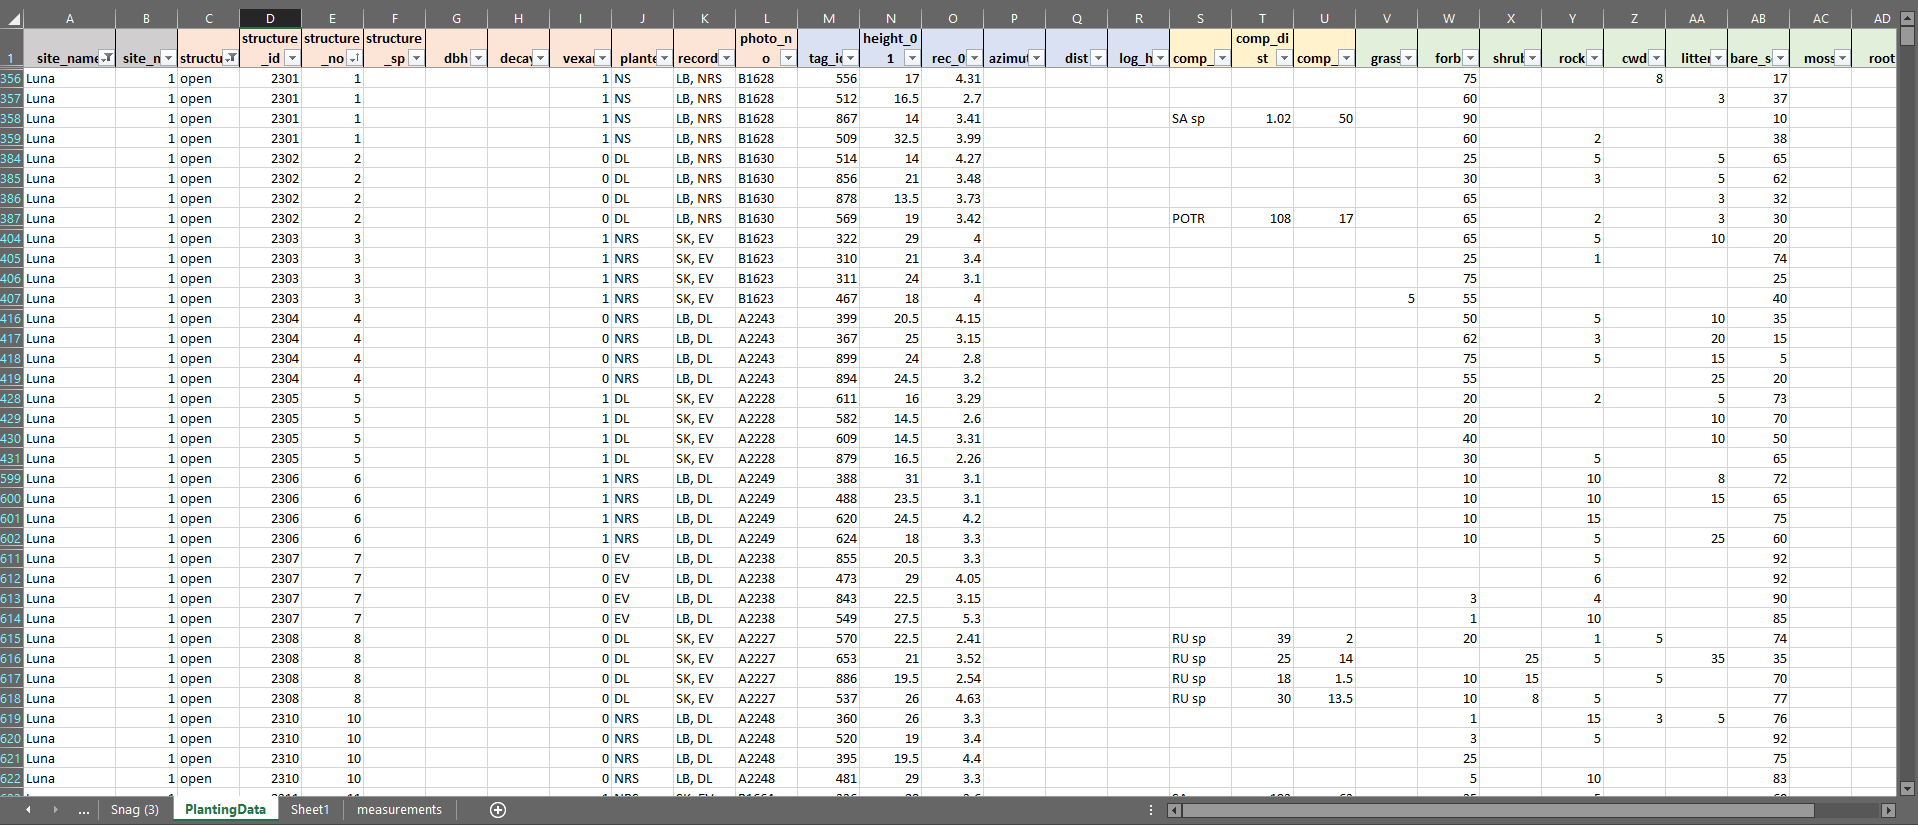
\includegraphics{old_data.png}
\caption{Fig. 1: Diagram of database structure}
\end{figure}

I color coded objects, merged cells, and had multiple sheets.

\hypertarget{my-new-data}{%
\subsection{My new data}\label{my-new-data}}

From this class, I learned the error in my ways and I quickly remade my
datasheets..

Here is a screenshot of my new data.

\begin{figure}
\centering
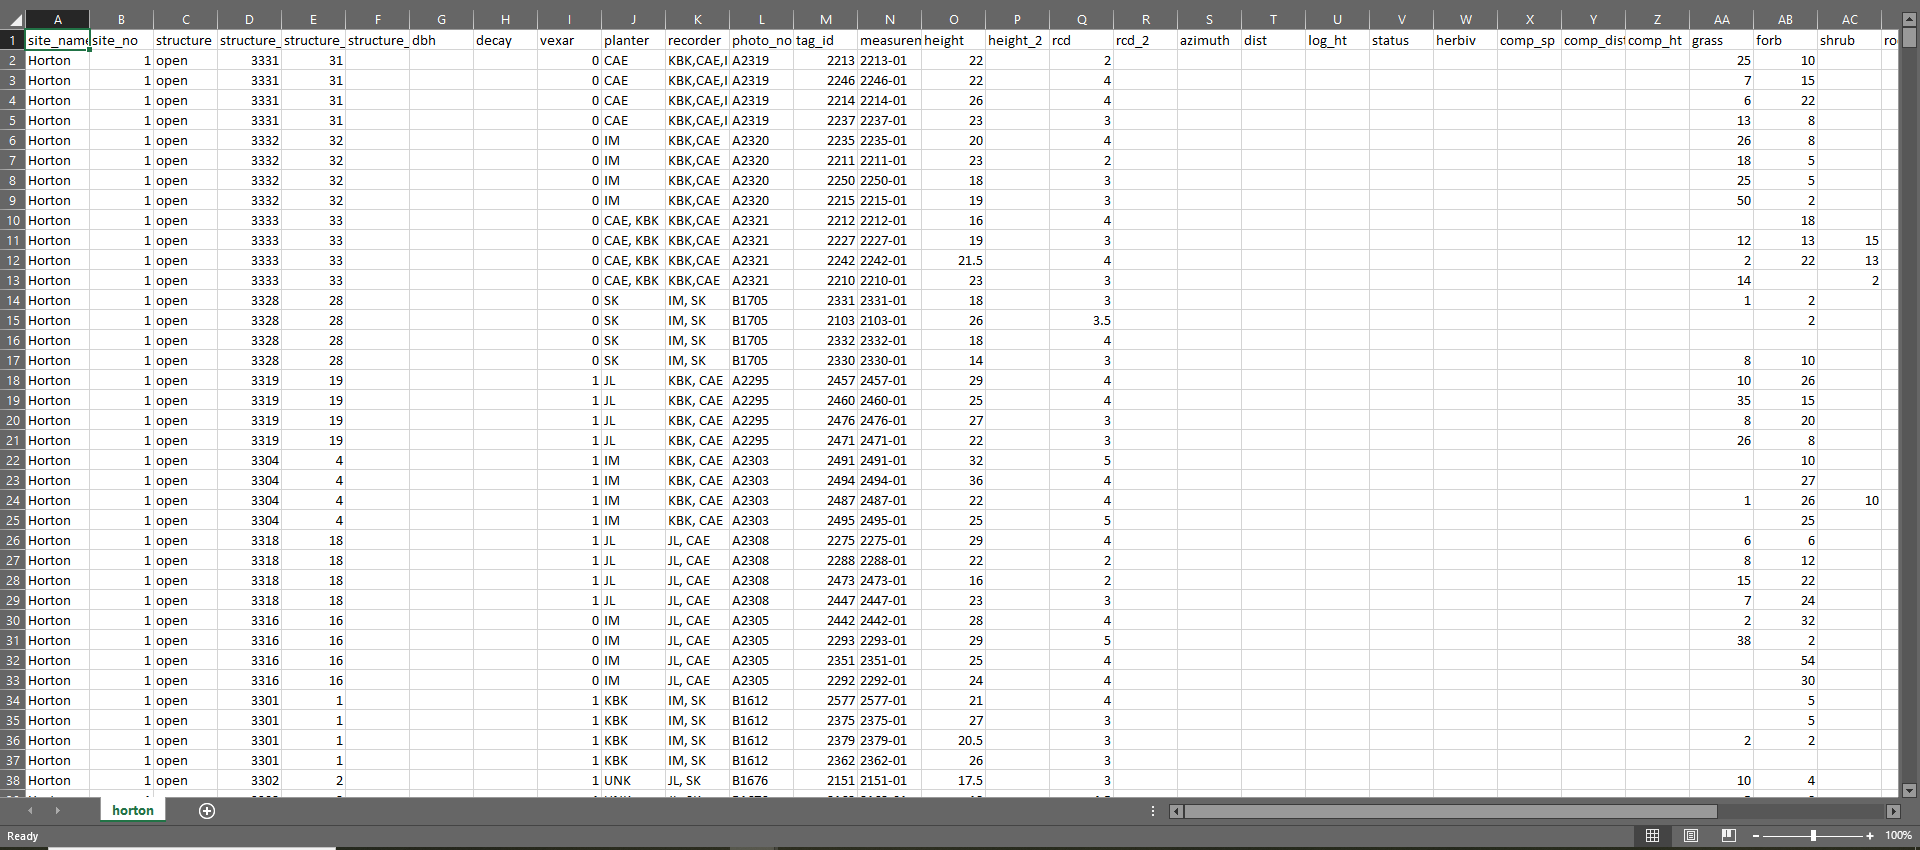
\includegraphics{new_data.png}
\caption{Fig. 1: Diagram of database structure}
\end{figure}

First, I used csv instead of excel since that is better compatible with R.
I removed any color coding since that will not translate in R. I also removed
merged cells since that will cause issues working in R. I also separated all
pages from the one excel file into various single page csv documents.

\hypertarget{building-the-aspen-seedling-database}{%
\chapter{Building the aspen seedling database}\label{building-the-aspen-seedling-database}}

\hypertarget{database-structure}{%
\section{Database structure}\label{database-structure}}

I will be constructing a database to organize my data. I have roughly 1,000 seedlings planted in four sites under three treatments across the Southwest. For this project, I will follow this database structure.

\begin{figure}

{\centering 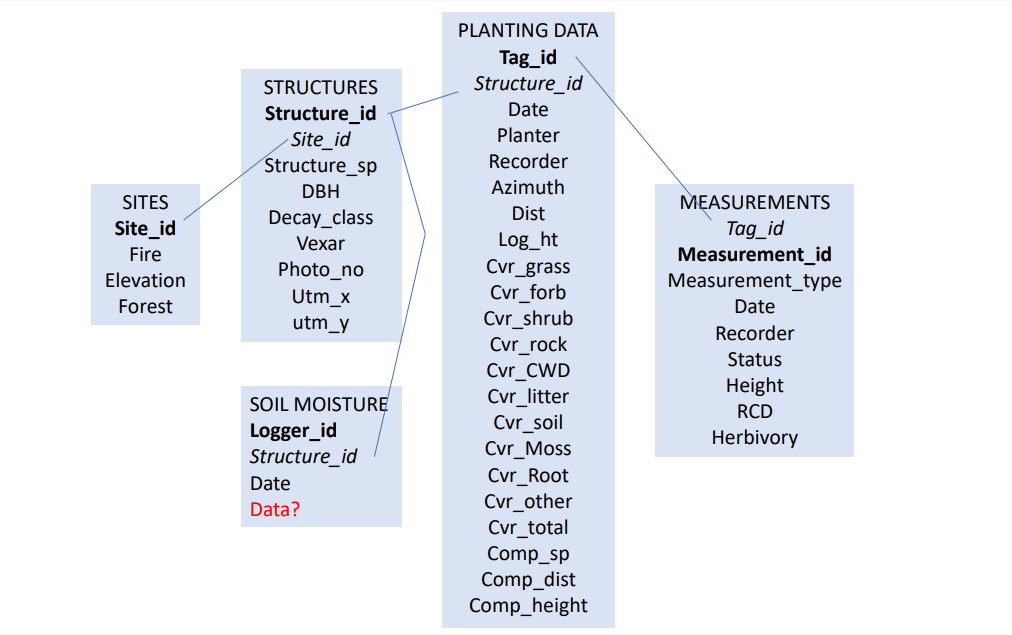
\includegraphics[width=1\linewidth]{database_structure} 

}

\caption{Diagram illustrating the structure of the database}\label{fig:diagram}
\end{figure}

\hypertarget{creating-the-database}{%
\section{Creating the database}\label{creating-the-database}}

This is the code we used to create the database. We'll start with loading our packages. I will need `DBI' and `RSQLite' packages. I will also download some other packages that might be of use later on.

\begin{Shaded}
\begin{Highlighting}[]
\FunctionTok{library}\NormalTok{(DBI)}
\FunctionTok{library}\NormalTok{(RSQLite)}
\FunctionTok{library}\NormalTok{(ggplot2)}
\FunctionTok{library}\NormalTok{(tidyverse)}
\FunctionTok{library}\NormalTok{ (lubridate)}
\end{Highlighting}
\end{Shaded}

First, we're going to start by establishing a connection to a SQLite database.

\begin{Shaded}
\begin{Highlighting}[]
\NormalTok{aspen\_db }\OtherTok{\textless{}{-}} \FunctionTok{dbConnect}\NormalTok{(RSQLite}\SpecialCharTok{::}\FunctionTok{SQLite}\NormalTok{())}
\end{Highlighting}
\end{Shaded}

\hypertarget{creating-the-measurements-table}{%
\subsection{Creating the measurements table}\label{creating-the-measurements-table}}

This table includes all baseline-measurement information about each seedling across all three fire footprints. I do not have information from repeat measurements yet. The table includes columns for tag id, measurement id, date, height of seedlings, root collar diameter of seedlings, site information, recorder information, survivorship status, and herbivory status. The primary key is the measurement id which will reflect when the measurement was done.

\begin{Shaded}
\begin{Highlighting}[]
\FunctionTok{dbExecute}\NormalTok{(aspen\_db, }\StringTok{"CREATE TABLE measurements (}
\StringTok{tag\_id varchar(4) NOT NULL,}
\StringTok{measurement\_id varchar (5) NOT NULL,}
\StringTok{date varchar (10), }
\StringTok{height varchar (4), }
\StringTok{rcd varchar (4),}
\StringTok{site\_name varchar, }
\StringTok{structure\_id varchar (2),}
\StringTok{structure\_type varchar (1),}
\StringTok{recorder varchar (10), }
\StringTok{status varchar (5),}
\StringTok{herbivory varchar (1),}
\StringTok{PRIMARY KEY (measurement\_id)}
\StringTok{);"}\NormalTok{)}

\NormalTok{measurements }\OtherTok{\textless{}{-}} \FunctionTok{read.csv}\NormalTok{(}\StringTok{"measurements.csv"}\NormalTok{,}\AttributeTok{stringsAsFactors =} \ConstantTok{FALSE}\NormalTok{)}

\FunctionTok{dbWriteTable}\NormalTok{(aspen\_db, }\StringTok{"measuremements"}\NormalTok{, measurements, }\AttributeTok{append =} \ConstantTok{TRUE}\NormalTok{)}
\end{Highlighting}
\end{Shaded}

\hypertarget{creating-the-sites-table}{%
\subsection{Creating the sites table}\label{creating-the-sites-table}}

This table includes information about each site within the three fire footprints. There are four sites total. The table includes columns for fire footprint, site id, elevation, and forest name. The primary key is the fire.

\begin{Shaded}
\begin{Highlighting}[]
\FunctionTok{dbExecute}\NormalTok{(aspen\_db, }\StringTok{"CREATE TABLE sites (}
\StringTok{fire varchar (9), }
\StringTok{site\_id varchar (1), }
\StringTok{elevation varchar (5), }
\StringTok{forest varchar (16),}
\StringTok{PRIMARY KEY (site\_id)}
\StringTok{);"}\NormalTok{)}

\NormalTok{sites }\OtherTok{\textless{}{-}} \FunctionTok{read.csv}\NormalTok{(}\StringTok{"sites.csv"}\NormalTok{,}\AttributeTok{stringsAsFactors =} \ConstantTok{FALSE}\NormalTok{)}

\FunctionTok{dbWriteTable}\NormalTok{(aspen\_db, }\StringTok{"sites"}\NormalTok{, sites, }\AttributeTok{append =} \ConstantTok{TRUE}\NormalTok{)}
\end{Highlighting}
\end{Shaded}

\hypertarget{creating-the-soil-moisture-table}{%
\subsection{Creating the soil moisture table}\label{creating-the-soil-moisture-table}}

This table includes information from the soil moisture sensors that will be installed in the Luna fire footprint. There is a column for logger\_id, structure\_id, and date. The logger id is the primary key. Since I don't know what this data will include and look like, it is empty for now.

\begin{Shaded}
\begin{Highlighting}[]
\FunctionTok{dbExecute}\NormalTok{(aspen\_db, }\StringTok{"CREATE TABLE soil\_moisture (}
\StringTok{logger\_id varchar (10), }
\StringTok{structure\_id varchar (3), }
\StringTok{date varchar (10),}
\StringTok{PRIMARY KEY (logger\_id)}
\StringTok{);"}\NormalTok{)}

\NormalTok{soil\_moisture }\OtherTok{\textless{}{-}} \FunctionTok{read.csv}\NormalTok{(}\StringTok{"soil\_moisture.csv"}\NormalTok{, }\AttributeTok{stringsAsFactors =} \ConstantTok{FALSE}\NormalTok{)}

\FunctionTok{dbWriteTable}\NormalTok{(aspen\_db, }\StringTok{"soil\_moisture"}\NormalTok{, soil\_moisture, }\AttributeTok{append =} \ConstantTok{TRUE}\NormalTok{)}
\end{Highlighting}
\end{Shaded}

\hypertarget{creating-the-structures-table}{%
\subsection{Creating the structures table}\label{creating-the-structures-table}}

This table includes information about each structure (or treatment) across all three fire footprints. There are columns for site name, site number, structure number, structure type, structure species (applicable for snags and logs), diameter at breast height (applicable for snags), decay class (applicable for snags and logs), vexar, photo number, and the utm coordinates. The primary key will be the photo number since each structure has it's own photo.

\begin{Shaded}
\begin{Highlighting}[]
\FunctionTok{dbExecute}\NormalTok{(aspen\_db, }\StringTok{"CREATE TABLE structures (}
\StringTok{site\_name varchar, }
\StringTok{site\_no varchar (1), }
\StringTok{structure\_no varchar (2),}
\StringTok{structure\_type varchar (1),}
\StringTok{structure\_sp varchar (5), }
\StringTok{dbh varchar (4), }
\StringTok{decay\_class varchar (1), }
\StringTok{vexar varchar (1),}
\StringTok{photo\_no varchar (6), }
\StringTok{utm\_x varchar (15), }
\StringTok{utm\_y varchar (15),}
\StringTok{PRIMARY KEY (photo\_no)}
\StringTok{);"}\NormalTok{)}

\NormalTok{structures }\OtherTok{\textless{}{-}} \FunctionTok{read.csv}\NormalTok{(}\StringTok{"structures.csv"}\NormalTok{, }\AttributeTok{stringsAsFactors =} \ConstantTok{FALSE}\NormalTok{)}

\FunctionTok{dbWriteTable}\NormalTok{(aspen\_db, }\StringTok{"structures"}\NormalTok{, structures, }\AttributeTok{append =} \ConstantTok{TRUE}\NormalTok{)}
\end{Highlighting}
\end{Shaded}

\hypertarget{database-is-complete}{%
\chapter{Database is complete}\label{database-is-complete}}

Yay! I have successfully created an aspen database. This will not be necessary for my research project moving forward. However, this experience was valuable to help me organize my thoughts and figure out the best way to compartmentalize my data.

\hypertarget{simulating-data-and-using-ggplot}{%
\chapter{Simulating data and using ggplot}\label{simulating-data-and-using-ggplot}}

In this chapter, I will show how I used simulated data to visualize some ``fake''
findings.

\hypertarget{simulating-the-data}{%
\section{Simulating the data}\label{simulating-the-data}}

First I simulated data to run. Below is very simple code I used to create
some data. I first manipulated the data using a binomial distribution. This
randomly selected some seedlings to survive and some to die. Of those that
survived, I increased the height by 40\% and the RCD by 30\%. Then I manually
added more weight to the snag treatment.

\begin{Shaded}
\begin{Highlighting}[]
\CommentTok{\# load packages }

\FunctionTok{library}\NormalTok{(tidyverse)}
\FunctionTok{library}\NormalTok{(lme4)}

\NormalTok{horton\_man }\OtherTok{\textless{}{-}} \FunctionTok{read.csv}\NormalTok{(}\StringTok{"horton\_man.csv"}\NormalTok{) }\SpecialCharTok{\%\textgreater{}\%}
  \FunctionTok{filter}\NormalTok{(}\FunctionTok{is.na}\NormalTok{(site\_no)}\SpecialCharTok{==} \ConstantTok{FALSE}\NormalTok{)}

\CommentTok{\# this is remnant code on how I did that: }
\CommentTok{\# horton\_man \textless{}{-} horton \%\textgreater{}\%}
  \CommentTok{\# mutate(measurement\_id = case\_when(tag\_id != "NA" \textasciitilde{}  paste0(tag\_id,"{-}02")),}
        \CommentTok{\# status = rbinom(n=350,prob = .75, size = 1),}
        \CommentTok{\# height = case\_when(status==1 \textasciitilde{} height*1.4, \# increase height by 40\%}
                          \CommentTok{\#  status==0 \textasciitilde{} height),}
        \CommentTok{\# rcd = case\_when(status == 1 \textasciitilde{} rcd*1.3, \# increase rcd by 30\%}
                        \CommentTok{\# status == 0 \textasciitilde{} rcd)) \%\textgreater{}\% }
  \CommentTok{\# filter(is.na(site\_no) == FALSE)}
\end{Highlighting}
\end{Shaded}

\hypertarget{plotting-the-data-using-ggplot}{%
\section{Plotting the data using ggplot}\label{plotting-the-data-using-ggplot}}

\hypertarget{plot-1}{%
\subsection{Plot 1}\label{plot-1}}

Below is the code I used to generate a bar plot displaying how many seedlings
survived in each treatment group. This is a simple plot but it does display what
treatment yielded the most seedling survival.

\begin{Shaded}
\begin{Highlighting}[]
\FunctionTok{library}\NormalTok{(ggplot2)}
\FunctionTok{library}\NormalTok{(viridis)}

\NormalTok{horton\_man }\SpecialCharTok{\%\textgreater{}\%} 
  \FunctionTok{as\_tibble}\NormalTok{() }\SpecialCharTok{\%\textgreater{}\%} 
  \FunctionTok{filter}\NormalTok{(status }\SpecialCharTok{==} \DecValTok{1}\NormalTok{) }\SpecialCharTok{\%\textgreater{}\%} 
  \FunctionTok{ggplot}\NormalTok{(}\FunctionTok{aes}\NormalTok{(}\AttributeTok{x =}\NormalTok{ structure, }\AttributeTok{fill =}\NormalTok{ status)) }\SpecialCharTok{+} 
  \FunctionTok{geom\_bar}\NormalTok{(}\AttributeTok{fill =} \StringTok{"light blue"}\NormalTok{) }\SpecialCharTok{+} 
  \FunctionTok{labs}\NormalTok{ (}\AttributeTok{x =} \StringTok{"Treatment"}\NormalTok{, }\AttributeTok{y =} \StringTok{"Count"}\NormalTok{,}
        \AttributeTok{title =} \StringTok{"Seedling Survival by Treatment"}\NormalTok{) }\SpecialCharTok{+} 
  \FunctionTok{theme\_light}\NormalTok{() }
\end{Highlighting}
\end{Shaded}

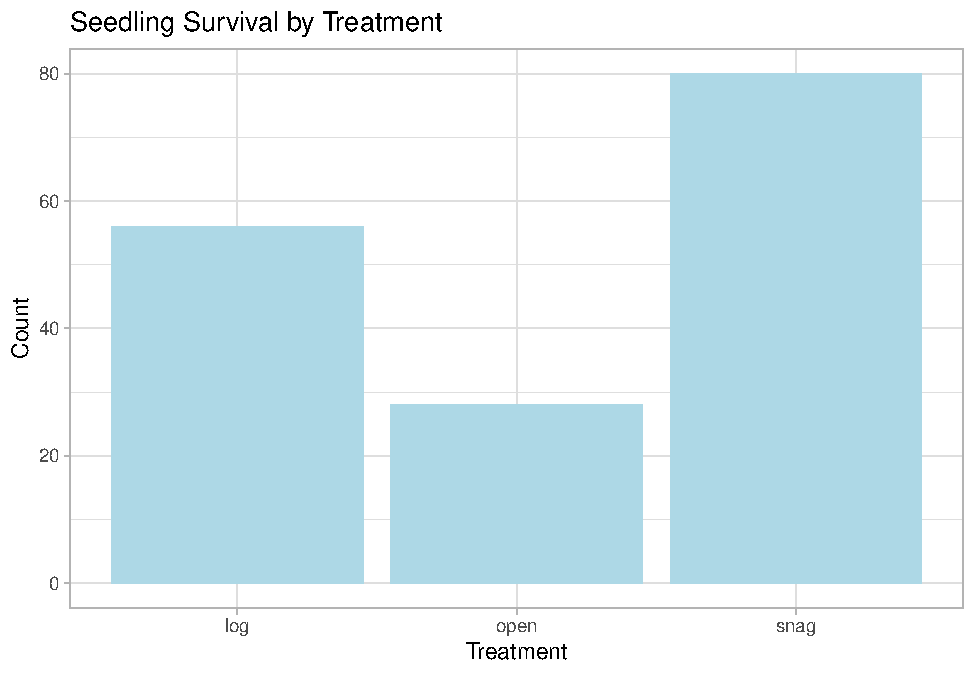
\includegraphics{_main_files/figure-latex/ggplot-1.pdf}
\#\#\# Plot 2

Below is code I used to plot the root collar diameter and height of each
seedling in the Horton fire. I wanted to compare growth of those that survive
from the time of planting to the second year.

\begin{Shaded}
\begin{Highlighting}[]
\FunctionTok{library}\NormalTok{(viridis)}
\FunctionTok{library}\NormalTok{(patchwork)}

\NormalTok{p1 }\OtherTok{\textless{}{-}}\NormalTok{ horton\_man }\SpecialCharTok{\%\textgreater{}\%} 
  \FunctionTok{as\_tibble}\NormalTok{() }\SpecialCharTok{\%\textgreater{}\%} 
  \FunctionTok{filter}\NormalTok{(status }\SpecialCharTok{==} \DecValTok{1}\NormalTok{) }\SpecialCharTok{\%\textgreater{}\%} 
  \FunctionTok{ggplot}\NormalTok{(}\FunctionTok{aes}\NormalTok{(}\AttributeTok{x =}\NormalTok{ rcd, }\AttributeTok{y =}\NormalTok{ height, }\AttributeTok{color =}\NormalTok{ tag\_id)) }\SpecialCharTok{+} 
  \FunctionTok{geom\_point}\NormalTok{(}\AttributeTok{alpha =} \FloatTok{0.7}\NormalTok{)}\SpecialCharTok{+}
  \FunctionTok{facet\_wrap}\NormalTok{(}\SpecialCharTok{\textasciitilde{}}\NormalTok{structure) }\SpecialCharTok{+}
  \FunctionTok{labs}\NormalTok{(}\AttributeTok{x =} \StringTok{"Root Collar Diameter (mm)"}\NormalTok{, }
       \AttributeTok{y =} \StringTok{"Height to Terminal Bud (mm)"}\NormalTok{, }
       \AttributeTok{title =} \StringTok{"Year 1"}\NormalTok{) }\SpecialCharTok{+}
  \FunctionTok{theme\_light}\NormalTok{() }\SpecialCharTok{+} 
  \FunctionTok{theme}\NormalTok{(}\AttributeTok{legend.position =} \StringTok{"none"}\NormalTok{) }\SpecialCharTok{+}  
  \FunctionTok{scale\_fill\_viridis}\NormalTok{(}\AttributeTok{option =} \StringTok{"magma"}\NormalTok{) }

\NormalTok{p2 }\OtherTok{\textless{}{-}}\NormalTok{ horton\_man }\SpecialCharTok{\%\textgreater{}\%} 
  \FunctionTok{as\_tibble}\NormalTok{() }\SpecialCharTok{\%\textgreater{}\%} 
  \FunctionTok{filter}\NormalTok{(status }\SpecialCharTok{==} \DecValTok{1}\NormalTok{) }\SpecialCharTok{\%\textgreater{}\%} 
  \FunctionTok{ggplot}\NormalTok{(}\FunctionTok{aes}\NormalTok{(}\AttributeTok{x =}\NormalTok{ rcd\_2, }\AttributeTok{y =}\NormalTok{ height\_2, }\AttributeTok{color =}\NormalTok{ tag\_id)) }\SpecialCharTok{+} 
  \FunctionTok{geom\_point}\NormalTok{(}\AttributeTok{alpha =} \FloatTok{0.7}\NormalTok{)}\SpecialCharTok{+}
  \FunctionTok{facet\_wrap}\NormalTok{(}\SpecialCharTok{\textasciitilde{}}\NormalTok{structure) }\SpecialCharTok{+}
  \FunctionTok{labs}\NormalTok{(}\AttributeTok{x =} \StringTok{"Root Collar Diameter (mm)"}\NormalTok{, }
       \AttributeTok{y =} \StringTok{"Height to Terminal Bud (mm)"}\NormalTok{, }
       \AttributeTok{title =} \StringTok{"Year 2"}\NormalTok{) }\SpecialCharTok{+}
  \FunctionTok{theme\_light}\NormalTok{() }\SpecialCharTok{+} 
  \FunctionTok{theme}\NormalTok{(}\AttributeTok{legend.position =} \StringTok{"none"}\NormalTok{) }\SpecialCharTok{+}  
  \FunctionTok{scale\_fill\_viridis}\NormalTok{(}\AttributeTok{option =} \StringTok{"magma"}\NormalTok{) }

\NormalTok{p1 }\SpecialCharTok{|}\NormalTok{ p2}
\end{Highlighting}
\end{Shaded}

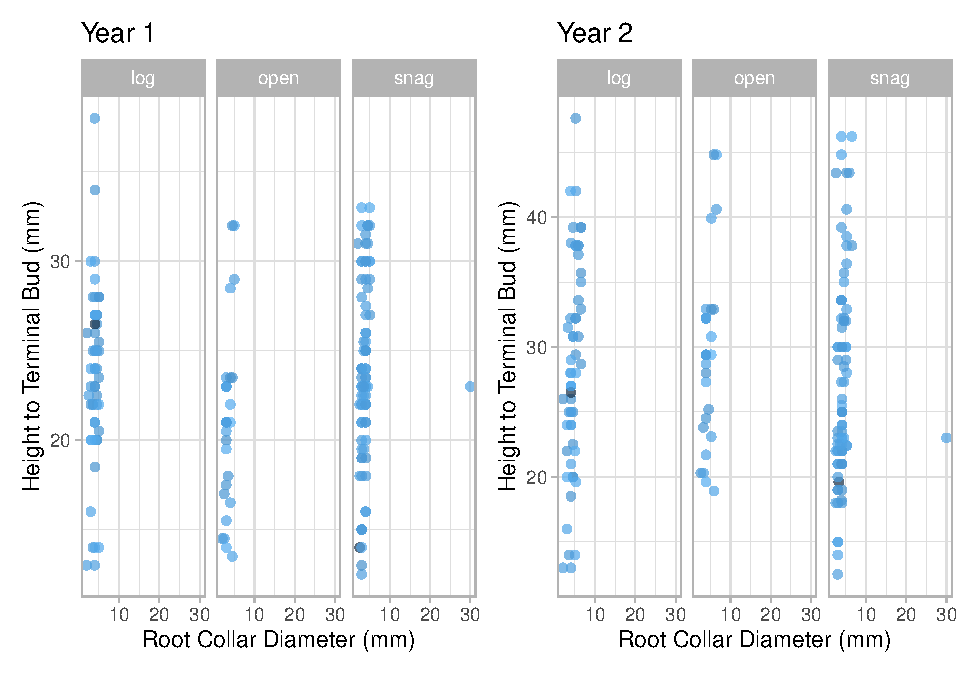
\includegraphics{_main_files/figure-latex/ggplot2-1.pdf}

  \bibliography{book.bib,packages.bib}

\end{document}
